\cabecalho

\section*{Exercício}

% Aula - \textit{20 de maio de 2026}

\begin{enumerate}
    \item Dimensione a viga $AB$ usando aço AR 350 COR, as cargas já estão majoradas escolha um perfil VS. % Considere apenas momento e cortante.
    
    
    
    \begin{tikzpicture}[
        % 1. DEFINIÇÃO DO SEU LIMITADOR CUSTOMIZADO (+ com /)
        cota customizada/.style={
            decoration={
            markings,
            mark=at position 0 with {
                \draw[thick] (-3.5pt, 0) -- (3.5pt, 0);          % Linha horizontal do +
                \draw[thick] (0, -3.5pt) -- (0, 3.5pt);          % Linha vertical do +
                \draw[thick] (-3.5pt, -3.5pt) -- (3.5pt, 3.5pt); % Linha diagonal
            },
            mark=at position 1 with {
                \draw[thick] (-3.5pt, 0) -- (3.5pt, 0);          % Linha horizontal do +
                \draw[thick] (0, -3.5pt) -- (0, 3.5pt);          % Linha vertical do +
                \draw[thick] (-3.5pt, -3.5pt) -- (3.5pt, 3.5pt); % Linha diagonal
            }
            },
            postaction={decorate} % Aplica o desenho nas pontas da linha
        }
        ]
        
        % VARIÁVEIS
        \def\L{12} % Comprimento total da viga

        % DESENHO DA VIGA
        \draw[thick] (0, 0) rectangle (\L, 0);

        % APOIOS
        % Apoio A (Fixo)
        \draw[thick] (0, 0) -- (-0.3, -0.5) -- (0.3, -0.5) -- cycle;
        \draw[thick] (-0.5, -0.6) -- (0.5, -0.6);
        %\foreach \x in {-0.4, -0.2, 0, 0.2, 0.4}
        %    \draw (\x, -0.5) -- (\x-0.2, -0.7);

        % Apoio B (Fixo)
        \draw[thick] (\L, 0) -- (\L-0.3, -0.5) -- (\L+0.3, -0.5) -- cycle;
        \draw[thick] (\L-0.5, -0.6) -- (\L+0.5, -0.6);
        %\foreach \x in {\L-0.4, \L-0.2, \L, \L+0.2, \L+0.4}
        %    \draw (\x, -0.5) -- (\x-0.2, -0.7);

        % Apoio B (Móvel)
        %\draw[thick] (\L, 0) -- (\L-0.3, -0.4) -- (\L+0.3, -0.4) -- cycle;
        %\draw[thick] (\L-0.5, -0.5) -- (\L+0.5, -0.5);
        
        % Rótulos
        \node[above] at (0, 0.2) {$A$};
        \node[above] at (\L, 0.2) {$B$};

        % CARGA CONCENTRADA (P)
        \draw[-{Latex[length=4mm]}, ultra thick, azul] (3, 1.5) -- (3, 0.1) 
            node[at start, above, text=black] {$6882 \ kN$};

        \draw[-{Latex[length=4mm]}, ultra thick, azul] (7, 1.5) -- (7, 0.1) 
            node[at start, above, text=black] {$2550 \ kN$};


        % Cota total
        \draw[cota customizada] (0, -2.5) -- (\L, -2.5) 
            node[midway, fill=white] {$12 \ m$};
            
        % Cotas parciais
        \draw[cota customizada] (0, -1.5) -- (3, -1.5) 
            node[midway, fill=white] {$3 \ m$};
            
        \draw[cota customizada] (3, -1.5) -- (7, -1.5) 
            node[midway, fill=white] {$4 \ m$};
            
        \draw[cota customizada] (7, -1.5) -- (\L, -1.5) 
            node[midway, fill=white] {$5 \ m$};

    \end{tikzpicture}

    \textcolor{gray}{\textbf{Reações de apoio e esforços solicitantes}}

    \textcolor{gray}{$\sum M_B = 0 \newline -12 V_A + 9 \cdot 6882 + 5 \cdot 2550 = 0 \newline V_A = 6224 \ kN$}

    \textcolor{gray}{$\sum F_y = 0 \newline V_A + V_B - 6882 - 2550 = 0 \newline V_B = 3208 \ kN$}

    

    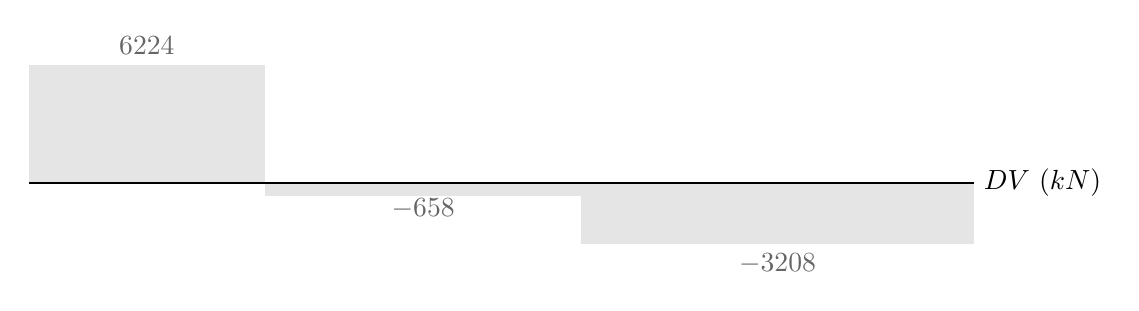
\begin{tikzpicture}
        % 1. VARIÁVEIS (Mantendo as mesmas proporções da viga anterior)
        \def\L{12}    % Comprimento total do diagrama (eixo x)
        \def\V{1.5}  % Altura do gráfico (representando a magnitude P/2)

        % 3. EIXO DE REFERÊNCIA (y = 0)
        % Linha que passa um pouco dos limites para indicar o eixo
        \draw[thick, gray] (0, 0) -- (\L, 0) node[right, text=black] {$DV \ (kN)$};

        % ==========================================
        % 4. ESFORÇO CORTANTE POSITIVO (0 até L/2)
        % ==========================================
        % Preenchimento com azul claro (20% de tinta azul, 80% branco)
        \fill[gray!20] (0,0) rectangle (\L/4, \V);

        % Rótulos da área positiva (Sinal de + e o valor P/2)
        \node[above, gray!80!black] at (\L/8, \V) {$6224$};

        % ==========================================
        % 5. ESFORÇO CORTANTE NEGATIVO (L/2 até L)
        % ==========================================
        % Preenchimento com vermelho claro
        \fill[gray!20] (\L/4,0) rectangle (\L/1.71, -0.11*\V);
        
        % Rótulos da área negativa (Sinal de - e o valor -P/2)
        \node[below, gray!80!black] at ({(\L/4 + \L/1.71)/2}, -0.11*\V/2) {$-658$};

        
        
        % Preenchimento com vermelho claro
        \fill[gray!20] (\L/1.71,0) rectangle (\L, -0.52*\V);
        
        % Rótulos da área negativa (Sinal de - e o valor -P/2)
        \node[below, gray!80!black] at ({(\L/1.71 + \L)/2}, -0.52*\V) {$-3208$};
        
        
        % Remarcando a linha base do diagrama em preto
        \draw[thick, black] (0,0) -- (\L,0);
    \end{tikzpicture}

    \textcolor{gray}{$V_{Sd,max} = V_A = 6224 \ kN$}

    

    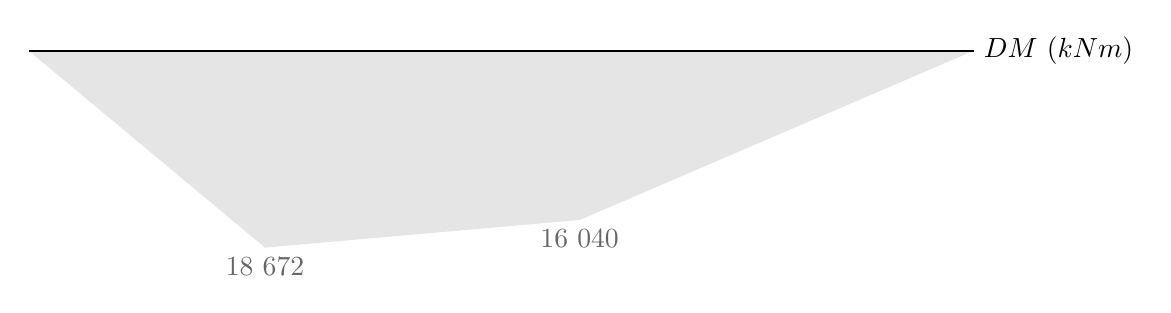
\begin{tikzpicture}
        % 1. VARIÁVEIS
        \def\L{12}   % Comprimento total da viga (eixo x)
        \def\V{2.5}  % Altura máxima do gráfico (representando os 40 kNm)

        % ==========================================
        % 2. EIXO DE REFERÊNCIA
        % ==========================================
        \draw[thick, gray] (0, 0) -- (\L, 0) node[right, text=black] {$DM \ (kNm)$};

        % ==========================================
        % 3. PREENCHIMENTO E CONTORNO PROPORCIONAL
        % ==========================================
        % Altura Y = 100% de \V (referente aos 40 kNm)
        % Posição X = 4m é um terço de L (\L/3) e 8m são dois terços (2*\L/3)
        \fill[gray!20] (0,0) -- (0.25*\L, -\V) -- (0.583*\L, -0.86*\V) -- (\L, 0) -- cycle;
        
        % Reforça a linha do eixo central em preto
        \draw[thick, black] (0,0) -- (\L,0);

        % ==========================================
        % 4. RÓTULOS, VALORES E GUIAS
        % ==========================================
        % Valores do momento máximo posicionados na cota -\V
        \node[below, gray!80!black] at (0.25*\L, -\V) {$18 \ 672$};
        \node[below, gray!80!black] at (0.583*\L, -0.86*\V) {$16\ 040$};

    \end{tikzpicture}

    %\textcolor{gray}{$M_C^1 = 3  V_A = 18 \ 672 \ kNm$}

    %\textcolor{gray}{$M_C^2 = 5  V_B = 16\ 040 \ kNm$}

    \textcolor{gray}{$M_{Sd,max} = M_C^1 = 18 \ 672 \ kNm$}

    %\newpage

    \textcolor{gray}{\textbf{Propriedades do material e coeficiente}}

    \textcolor{gray}{AR 350 COR $\to f_y = 350 \ MPa, f_u = 485 \ MPa$ (Tabela A.1 da NBR 8800)}

    \textcolor{gray}{$\gamma_{a1} = 1,1$ (Tabela 3 da NBR 8800)}

    \textcolor{gray}{\textbf{Pré-dimensionamento à flexão}}

    \textcolor{gray}{$\lambda \leq \lambda_p$ (Anexo D.2.1 da NBR 8800)} 

    \textcolor{gray}{$M_{Sd} \leq M_{Rd}$ (Item 5.4.1.3 da NBR 8800) \newline $M_{Sd} \leq \frac{1}{\gamma_{a1}} M_{pl} \to M_{pl} = f_y W$ (Tabela D.1 da NBR 8800) \newline $W = \frac{M_{Sd} \cdot \gamma_{a1}}{f_y} \newline W = \frac{18\ 672 \cdot 10^3 \times 1,1}{350 \cdot 10^6} \newline W \approx 58,68 \cdot 10^{-3} \ m^3$}

    \textcolor{gray}{\textbf{Pré-dimensionamento ao cisalhamento}}

    \textcolor{gray}{$\lambda \leq \lambda_p$ (Anexo D.2.1 da NBR 8800)} 

    \textcolor{gray}{$V_{Sd} \leq V_{Rd}$ (Item 5.4.1.3 da NBR 8800) \newline $V_{Sd} \leq \frac{V_{pl}}{\gamma_{a1}} \to V_{pl} = 0,6 A_w f_y$ (Item 5.4.3.1.1, 5.4.3.1.2 da NBR 8800) \newline $A_w = \frac{V_{Sd} \times \gamma_{a1}}{0,6 f_y} \newline A_w = \frac{6224 \cdot 10^3 \times 1,1}{0,6 \times 350 \cdot 10^6} \newline A_w = 32,60 \cdot 10^{-3} \ m^2$}

    \textcolor{gray}{\textbf{Perfil VS}}

    \textcolor{gray}{$A_w = d \times t_w$ (Item 5.4.3.1.2 da NBR 8800) \newline $A_w = 1500 \cdot 10^{-3} \times 12,5 \cdot 10^{-3} \newline A_w = 18,75 \cdot 10^{-3} \ m^2$}

    \textcolor{gray}{$VS \ 1500 \times 492 \to W = 38950 \ cm^3, \ A = 18,75 \cdot 10^{-3} \ m^2$}

    \textcolor{gray}{$\therefore$ Não existe perfil VS capaz de suportar esse carregamento. Seria necessário projetar uma sob medida.}

    
    
    
    \newpage

    \textcolor{red}{\textbf{\MakeUppercase{Correção}}}

    \textcolor{gray}{\textbf{Pré dimensionamento à flexão}}

    \textcolor{gray}{$M_{Sd} \leq M_{Rd} \newline 18672 \cdot 10^3 \leq \frac{W \times 350 \cdot 10^6}{1,1} \newline W \approx 58,68 \cdot 10^{-3} \ m^3$}

    \textcolor{gray}{Perfil escolhido: VS $800 \times 143 \to Z = 5910 \ cm^3$}

    \textcolor{gray}{\textbf{FLM}}

    \textcolor{gray}{$\lambda \leq \lambda_p \newline \frac{b}{t} \leq 0,38 \sqrt{\frac{E}{fy}} \newline \frac{\frac{320 \cdot 10^{-3}}{2}}{19 \cdot 10^{-3}} \leq 0,38 \sqrt{\frac{200 \ 000 \cdot 10^6}{350 \cdot 10^6}} \newline 8,42 \leq 9,08$}

    \textcolor{gray}{$M_{Rd} = \frac{M_{pl}}{\gamma_{a1}} = \frac{5910 \times 35}{1,1} = 188045,45 \ kNcm$}

    \textcolor{gray}{\textbf{FLA}}

    \textcolor{gray}{$\lambda = \frac{h}{t_w} = \frac{76,2}{0,8} = 95,25$}

    \textcolor{gray}{$\lambda_p = 3,76 \sqrt{\frac{20000}{35}} = 89,88$}

    \textcolor{gray}{$\lambda_r = 5,7 \sqrt{\frac{20000}{35}} = 136,25$}

    \textcolor{gray}{$\lambda_p \leq \lambda < \lambda_r$}

    \textcolor{gray}{$M_r = w_x \times f_y = 5374 \times 35 = 188090 \ kNcm$}

    \textcolor{gray}{$M_{pl} = 206850 \ kNcm$}

    \textcolor{gray}{$M_{Rd} = \frac{1}{\gamma_{a1}} = (M_{pl}-(M_{pl}-M_r)\frac{\lambda-\lambda_p}{\lambda_r-\lambda_p}) = 186070,53 \ kNcm$}

    \textcolor{gray}{$\therefore$ Acontecerá flambagem na alma desse perfil.}





    \newpage

    \textcolor{gray}{\textbf{\MakeUppercase{Segunda tentativa}}}

    \textcolor{gray}{\textbf{FLM}}

    \textcolor{gray}{$0,35 \leq k_c \leq 0,76 \ \text{(Tabela 4, nota de rodapé a da Norma 8800)} \newline k_c = \frac{4}{\sqrt{\frac{h}{t_w}}} \newline k_c = \frac{4}{\sqrt{\frac{81,2}{0,8}}} \newline k_c = 0,397$}

    \textcolor{gray}{$\lambda_p < \lambda \leq \lambda_r \newline 0,38 \sqrt{\frac{E}{fy}} < \frac{b}{t} \leq 0,95 \sqrt{\frac{E}{(f_y - \sigma_r)/k_c}} \newline 0,38 \sqrt{\frac{200 \ 000 \cdot 10^6}{350 \cdot 10^6}} < \frac{\frac{350 \cdot 10^{-3}}{2}}{19 \cdot 10^{-3}} \leq 0,95 \sqrt{\frac{200\ 000 \cdot 10^6}{(350 \cdot 10^6 - \sigma_r)/0,397}}  \newline 9,08 < 9,21 \leq 17,10$}

    \textcolor{gray}{$M_{pl} = 6845 \times 35 = 2396 \ kNcm$}

    \textcolor{gray}{$M_r = 6243 \times 35 = 218505 \ kNcm$}

    \textcolor{gray}{$M_{Rd} = \frac{1}{\gamma_{a1}} = (M_{pl}-(M_{pl}-M_r)\frac{9,21-9,08}{17,12-9,08})= 217485 \ kNcm$}

    \textcolor{gray}{\textbf{FLA}}

    \textcolor{gray}{$\lambda = \frac{b}{t_w} = \frac{81,2}{0,8} = 101,5$}

    \textcolor{gray}{$\lambda_p = 89,88$}

    \textcolor{gray}{$\lambda_r = 136,25$}

    \textcolor{gray}{$M_{Rd} = \frac{1}{\gamma_{a1}} = (M_{pl}-(M_{pl}-M_r)\frac{9,21-9,08}{17,12-9,08}) = 212995 \ kNcm$}

    \textcolor{gray}{\textbf{FLT}}

    \textcolor{gray}{$\lambda = \frac{L_b}{r_y} = \frac{1200 \cdot 10^{-2}}{8,28 \cdot 10^{-2}} = 144,92$}

    \textcolor{gray}{$\lambda = 1,76 \sqrt{\frac{E}{f_y}} = 42,07$}

    \textcolor{gray}{$\lambda_r = \frac{1,38 c_b \sqrt{I_yJ}}{r_y \times J \times B_y} \sqrt{1+ \sqrt{\frac{1+27C_w B_1^2}{C_b^2}}}= 118$}

    \textcolor{gray}{$B_1 = \frac{(f_y - \sigma_r)W}{EJ} \newline B_1 = \frac{(\frac{70}{100}f_y) 6243}{20 \ 000 \times 174} \newline B_1 = 0,0439$}

    \textcolor{gray}{$C_w = \frac{I_y(d-t_y)^2}{4} \ \text{Para seções I} \newline C_w = \frac{13581(85-1,9)^2}{4} \newline C_w = 2344672,35$}

    \textcolor{gray}{$C_b d = \frac{12,5 M_{max}}{2,5M_{max}+3M_A+4M_B+3M_C}R_m  \to R_M =1 \newline C_b = \frac{12,5 \times 186720}{2,5 \times 186720+3 \times 186720 +4 \times 16698 +3 \times 9624}R_m \newline C_b = 1,176$}

    \textcolor{gray}{$M_{Rd} = \frac{1}{\gamma_{a1}} M_{Ce}$}

    \textcolor{gray}{$text$}

\end{enumerate}